\usetikzlibrary{arrows, shapes, positioning, shadows, trees}
\tikzset{
  basic/.style  = {draw, text width=2cm, drop shadow, font=\sffamily, rectangle},
  root/.style   = {basic, rounded corners=2pt, thin, align=center, fill=white},
  level 2/.style = {basic, rounded corners=6pt, thin,align=center, fill=white, text width=8em},
  level 3/.style = {basic, thin, align=left, fill=white, text width=6.5em}
}

\chapter{Marco Teórico}
% Lorem ipsum dolor sit amet, consectetur adipiscing elit. Sed vitae libero fermentum, consequat sem a, mattis magna. Mauris neque elit, varius hendrerit neque ut, elementum tempus nisi. Nulla in porttitor augue. Morbi ut turpis lorem. Phasellus porta feugiat dui, ut lacinia nisl. Nulla blandit ornare dolor, vel iaculis velit suscipit non. Morbi egestas ex eu mauris tempus, et fringilla enim tristique. Suspendisse potenti. Integer ut nibh lorem. Integer odio neque, suscipit vel ex commodo, congue aliquet dui.\\

% Maecenas lobortis purus at diam pellentesque, ut mollis sapien cursus. Etiam ultricies porta purus at tincidunt. Proin scelerisque erat sit amet hendrerit condimentum. Aenean quis leo molestie, tristique mauris id, facilisis dolor. Aliquam ornare sollicitudin dolor, nec pellentesque mauris laoreet vitae. In pulvinar commodo convallis. Ut ut venenatis enim, tincidunt elementum ante. Donec ut varius augue, faucibus vehicula massa. Proin placerat, augue porttitor semper laoreet, urna augue euismod leo, sit amet volutpat erat orci non dui. Nam lacinia nec felis quis tempor. Mauris eleifend at turpis nec efficitur.\\

\section{StressUN}
\textit{StressUN} es una libreria que hace uso de \textit{processing}\footnote{véase https://processing.org/} y \textit{frames}\footnote{véase https://github.com/VisualComputing/frames} como librerias. Se podría pensar a \textit{StressUN} como una aplicación específica de la libreria \textit{frames}. \\

La libreria tiene por objetivo ser un \textit{pre procesador} y \textit{pos procesador} en el análisis de estructuras conformadas por elementos tipo \textit{póritco}.\\

La libreria se divide en cuatro grupos de clases, como se muestra en la \ref{fig:modulosStressUN}, que son
\begin{itemize}
    \item \textit{constants},
    \item \textit{core},
    \item \textit{exceptions} y
    \item \textit{primitives}.
\end{itemize}

\begin{figure}[ht]
    \centering
    
    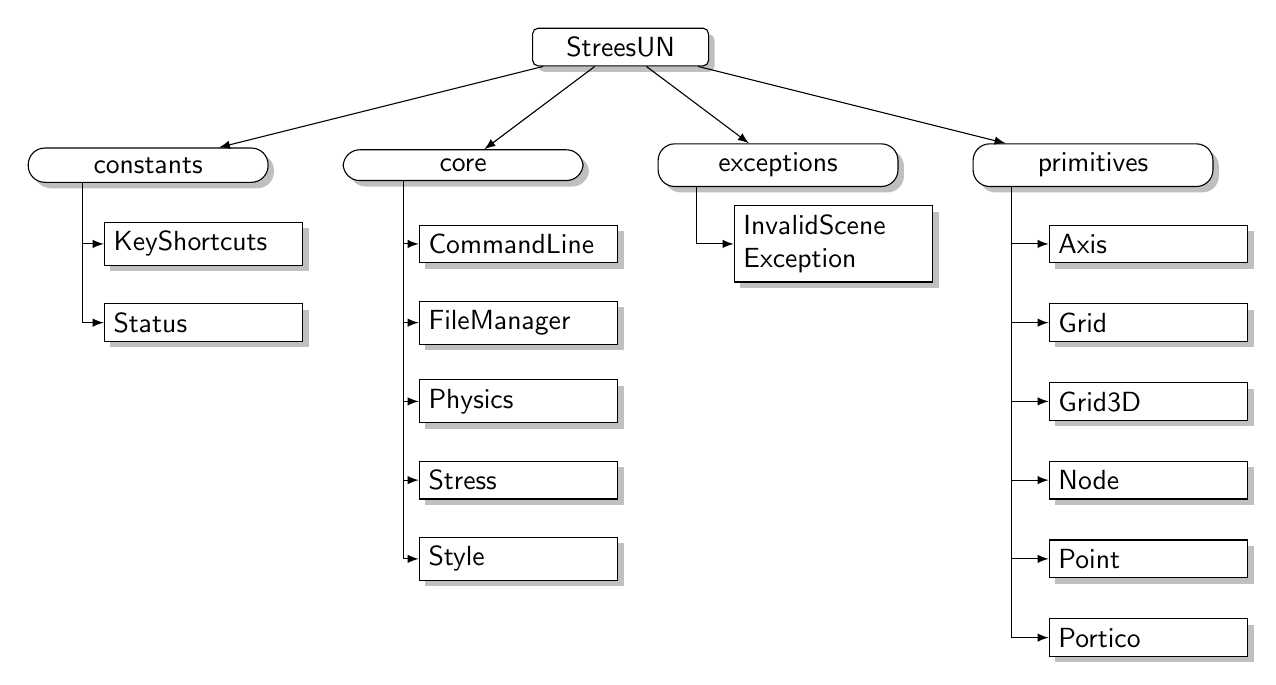
\begin{tikzpicture}[
        level 1/.style={sibling distance=40mm}, edge from parent/.style={->,draw}, >=latex]
        % root of the the initial tree, level 1
        \node[root] {StreesUN}
        % The first level, as children of the initial tree
        child {node[level 2] (c1) {constants}}
        child {node[level 2] (c2) {core}}
        child {node[level 2] (c3) {exceptions}}
        child {node[level 2] (c4) {primitives}};

        % The second level, relatively positioned nodes
        \begin{scope}[every node/.style={level 3}]
            \node [below of = c1, xshift=20pt] (c11) {KeyShortcuts};
            \node [below of = c11] (c12) {Status};

            \node [below of = c2, xshift=20pt] (c21) {CommandLine};
            \node [below of = c21] (c22) {FileManager};
            \node [below of = c22] (c23) {Physics};
            \node [below of = c23] (c24) {Stress};
            \node [below of = c24] (c25) {Style};

            \node [below of = c3, xshift=20pt] (c31) {InvalidScene
            Exception};
            
            \node [below of = c4, xshift=20pt] (c41) {Axis};
            \node [below of = c41] (c42) {Grid};
            \node [below of = c42] (c43) {Grid3D};
            \node [below of = c43] (c44) {Node};
            \node [below of = c44] (c45) {Point};
            \node [below of = c45] (c46) {Portico};
            
        \end{scope}

        % lines from each level 1 node to every one of its "children"
        \foreach \value in {1,2}
            \draw[->] (c1.195) |- (c1\value.west);

        \foreach \value in {1,...,5}
            \draw[->] (c2.195) |- (c2\value.west);

        \foreach \value in {1}
            \draw[->] (c3.195) |- (c3\value.west);
        
        \foreach \value in {1,...,6}
            \draw[->] (c4.195) |- (c4\value.west);
    \end{tikzpicture}
    
    \caption{Clases de la librería \textit{StressUN}.}
    \label{fig:modulosStressUN}
\end{figure}

\subsection{constants}
\subsubsection{KeyShortcuts}
Se almacenan los atajos de teclado que el usuario tiene a disposición.
\subsubsection{Status}
Se almecena el el estado del programa, el cual varia entre el \textit{canvas}, el \textit{command line} y el \textit{menu}.

\subsection{core}
\subsubsection{CommandLine}
Recibe los comandos por teclado
\subsubsection{FileManager}
Administra los archivos que contienen la información del modelo.
\subsubsection{Physics}
Proceso.
\subsubsection{Stress}
Administra las demás clases.
\subsubsection{Style}
Admisnitra los estilos del \textit{pre proceso} y del \textit{pos proceso}.

\subsection{excepetions}
\subsubsection{InvalidSceneException}
Generar un error si no se usa \textit{P3D}.

\subsection{primitives}
\subsubsection{Axis}
Ejes de la estructura.
\subsubsection{Grid}
Conjunto de ejes en un mismo plano.
\subsubsection{Grid3D}
Conjunto de grids.
\subsubsection{Node}
Extremo de un elemento tipo portico.
\subsubsection{Point}
Sirve como snap.
\subsubsection{Portico}
Elemento de la estructura.

% \subsection{Subt\'{\i}tulos nivel 3}
% De la cuarta subdivisi\'{o}n en adelante, cada nueva divisi\'{o}n o \'{\i}tem puede ser se\~{n}alada con vi\~{n}etas, conservando el mismo estilo de \'{e}sta, a lo largo de todo el documento.\\

% Las subdivisiones, las vi\~{n}etas y sus textos acompa\~{n}antes deben presentarse sin sangr\'{\i}a y justificados.\\

% \begin{itemize}
% \item En caso que sea necesario utilizar vi\~{n}etas, use este formato (vi\~{n}etas cuadradas).
% \end{itemize}